\documentclass{article}
\usepackage{hyperref,amsmath,amssymb}
\usepackage{tikz,comment}
\usetikzlibrary{automata, arrows.meta, positioning,decorations.pathmorphing}

\begin{document}

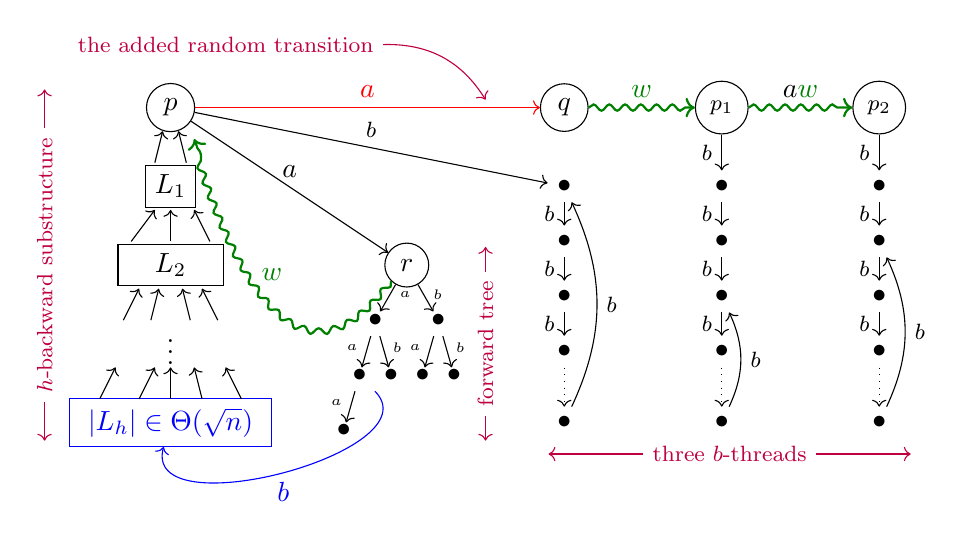
\begin{tikzpicture}
	\node[draw, circle] (s) at (0,0) {$p$};
	
	% s backward tree
	\node[draw] (b1) at (0,-1) {$L_1$};
	\node[draw] (b2) at (0,-2) {$\quad L_2\quad$};
	\node (dots1) at (0,-3) {$\vdots$};
	\node[draw,blue] (btau) at (0,-4) {$\ |L_h|\in\Theta(\sqrt{n})\ $};

	\draw[->] (.2,-0.7) -- (.1,-0.3);
	\draw[->] (-.2,-0.7) -- (-.1,-0.3);
	
	\draw[->] (0,-1.7) -- (0,-1.3);
	\draw[->] (-.5,-1.7) -- (-.2,-1.3);
	\draw[->] (.5,-1.7) -- (.3,-1.3);

	\draw[->] (-.25,-2.7) -- (-.15,-2.3);
	\draw[->] (.25,-2.7) -- (.15,-2.3);
	\draw[->] (-.6,-2.7) -- (-.4,-2.3);
	\draw[->] (.6,-2.7) -- (.4,-2.3);
	
	\draw[->] (0,-3.7) -- (0,-3.3);
	\draw[->] (-.4,-3.7) -- (-.2,-3.3);
	\draw[->] (.4,-3.7) -- (.3,-3.3);
	\draw[->] (-.9,-3.7) -- (-.7,-3.3);
	\draw[->] (.9,-3.7) -- (.7,-3.3);

    	\draw[thin,<->,purple] (-1.6,-4.23) -- node[rotate=90,fill=white]{\footnotesize $h$-backward substructure} (-1.6,0.23);

	% r forward tree
	\node[draw,circle] (r) at (3,-2) {$r$};
	\draw[->] (s) -- node[above]{$a$} (r);
	\node(ra) at (2.6, -2.7) {$\bullet$}; \draw[->,shorten >=-3pt] (r) -- node[right]{\tiny $a$} (ra);
	\node (rb) at (3.4, -2.7) {$\bullet$}; \draw[->,shorten >=-3pt] (r) -- node[right]{\tiny $b$} (rb);
	\node (raa) at (2.4, -3.4) {$\bullet$}; \draw[->,shorten >=-3pt] (ra) -- node[left]{\tiny $a$} (raa);
	\node (rab) at (2.8, -3.4) {$\bullet$}; \draw[->,shorten >=-3pt] (ra) -- node[right]{\tiny $b$} (rab);
	\node (rba) at (3.2, -3.4) {$\bullet$}; \draw[->,shorten >=-3pt] (rb) -- node[left]{\tiny $a$} (rba);
	\node (rbb) at (3.6, -3.4) {$\bullet$}; \draw[->,shorten >=-3pt] (rb) -- node[right]{\tiny $b$} (rbb);
	\node (raaa) at (2.2, -4.1) {$\bullet$}; \draw[->,shorten >=-3pt] (raa) -- node[left]{\tiny $a$} (raaa);
	\draw[blue,->]  (raa) edge[bend left=120] node[below]{$b$} (btau);

	\draw[thin,<->,purple] (4,-4.23) -- node[rotate=90,fill=white]{\footnotesize forward tree} (4,-1.77);

	% added transition
	\node[draw,circle] (t) at (5,0) {$q$};
	\draw[->,red] (s) -- node[above]{$a$} (t);

	\node[draw,circle] (s1) at (7,0) {\footnotesize $p_1$};
	\draw[->,thick,green!50!black,decorate,decoration={snake,amplitude=.4mm,segment length=2mm,post length=1mm}] (t) -- node[above]{$w$} (s1);

	\node[draw,circle] (s2) at (9,0) {\footnotesize $p_2$};
	\draw[->,thick, green!50!black,decorate,decoration={snake,amplitude=.4mm,segment length=2mm,post length=1mm}] (s1) -- node[above]{${\color{black}a}w$} (s2);

	\draw[->,green!50!black, thick,decorate,decoration={snake,amplitude=.4mm,segment length=2mm,post length=1mm}] (2.8,-2.2) .. controls (1.3,-4.2) and  (.4,-.6) .. node[right]{$w$} (.3,-.4);
	
	\node (p01) at (5,-1) {$\bullet$}; \draw[->] (s) -- node[above]{\footnotesize $b$} (p01);
	\node (p02) at (5,-1.7) {$\bullet$}; \draw[->] (p01) -- node[left]{\footnotesize $b$} (p02);
	\node (p03) at (5,-2.4) {$\bullet$}; \draw[->] (p02) -- node[left]{\footnotesize $b$} (p03);
	\node (p04) at (5,-3.1) {$\bullet$}; \draw[->] (p03) -- node[left]{\footnotesize $b$} (p04);
	\node (p0n) at (5,-4) {$\bullet$}; \draw[->,dotted] (p04) -- (p0n);
	\draw[->] (p0n) edge[bend right=25] node[right]{\footnotesize $b$} (p01);

	\node (p11) at (7,-1) {$\bullet$}; \draw[->] (s1) -- node[left]{\footnotesize $b$} (p11);
	\node (p12) at (7,-1.7) {$\bullet$}; \draw[->] (p11) -- node[left]{\footnotesize $b$} (p12);
	\node (p13) at (7,-2.4) {$\bullet$}; \draw[->] (p12) -- node[left]{\footnotesize $b$} (p13);
	\node (p14) at (7,-3.1) {$\bullet$}; \draw[->] (p13) -- node[left]{\footnotesize $b$} (p14);
	\node (p1n) at (7,-4) {$\bullet$}; \draw[->,dotted] (p14) -- (p1n);
	\draw[->] (p1n) edge[bend right=25] node[right]{\footnotesize $b$} (p13);

	\node (p21) at (9,-1) {$\bullet$}; \draw[->] (s2) -- node[left]{\footnotesize $b$} (p21);
	\node (p22) at (9,-1.7) {$\bullet$}; \draw[->] (p21) -- node[left]{\footnotesize $b$} (p22);
	\node (p23) at (9,-2.4) {$\bullet$}; \draw[->] (p22) -- node[left]{\footnotesize $b$} (p23);
	\node (p24) at (9,-3.1) {$\bullet$}; \draw[->] (p23) -- node[left]{\footnotesize $b$} (p24);
	\node (p2n) at (9,-4) {$\bullet$}; \draw[->,dotted] (p24) -- (p2n);
	\draw[->] (p2n) edge[bend right=25] node[right]{\footnotesize $b$} (p22);

	\draw[thin,<->,purple] (4.8,-4.4) -- node[fill=white]{\footnotesize three $b$-threads} (9.4,-4.4);

    \node[purple] (text) at (.7,.8) {\footnotesize the added random transition};
    \draw[purple, thin] (text.east) edge[->,bend left] (4,.1);

	\end{tikzpicture}

\end{document}